\chapter{Fundamentação Teórica} \label{cap:cap2}

Este Capítulo relaciona os conceitos e as tecnologias envolvidas no desenvolvimento do ambiente de treinamento proposto. 

\section{Anestesias}

Anestesias são atualmente usadas em diversos procedimentos cirúrgicos na medicina tradicional com o intuito de bloquear temporariamente a capacidade do cérebro de reconhecer um estímulo doloroso. Esta prática visa permitir a execução de procedimentos invasivos por parte do médico enquanto mantém o conforto e a tranquilidade do paciente. Anestesias podem ter ação geral, regional ou local. Na anestesia geral é necessário agir no cérebro, impedindo que este reconheça os sinais de dor que recebe. Este tipo de anestesia é normalmente utilizado para efetuação de cirurgias de alto grau de complexidade que são feitas com o paciente inconsciente. Anestesias regionais são efetuadas na medula espinhal impedindo que sinais de dor vindo de nervos periféricos cheguem até o cérebro. Este tipo de anestesia é recomendado para cirurgias de menor complexidade onde o paciente permanece consciente. A anestesia regional bloqueia a dor em apenas uma determinada região do corpo, como um braço, uma perna ou toda região inferior do corpo, abaixo do abdômen. A anestesia local é o tipo de anestesia mais comum e ocorre através da atuação nos receptores da dor presentes na pele e nervos mais superficiais. Este tipo de anestesia, diferentemente das demais não é de administração restrita aos anestesistas como as demais. A anestesia local usualmente utilizada antes de uma anestesia regional através de injeção mas também pode ser feita através de gel ou spray em diferentes tipos de procedimentos onde é aplicada\cite{Pinheiro2018}.

Os dois tipos de anestesias regionais mais usados são: anestesia raquidiana e anestesia peridural ou epidural. Ambas podem ser aplicadas com pacientes sentados e inclinados para frente ou deitados de lado \cite{Anesclin2019}. Uma vez que estes dois tipos de anestesia possuem algumas similaridades iremos descrever os dois tipos aqui por que neste trabalho comparamos os simuladores existentes destes dois tipos de anestesia de forma a sermos mais abrangentes.  

Tanto na anestesia raquidiana quanto na peridural, após a finalização dos procedimentos de preparação é escolhida a área onde será feita a punção. Conforme já comentado anteriormente isto é comumente feito através da apalpação, que é o toque da mão do médico (Figura~\ref{fig:marcacaoPonto}) na crista ilíaca do paciente \cite{Helayel2010,Isaacs2015}. Uma vez escolhido este ponto é feita a injeção de anestésico local (Figura~\ref{fig:anestesiaLocal}) para reduzir o desconforto na área próxima à punção \cite{Sedicias2018} Após a anestesia local é feita a inserção da agulha de punção tanto no caso da peridural como na raqui.

\begin{figure}[ht!]
    \centering
    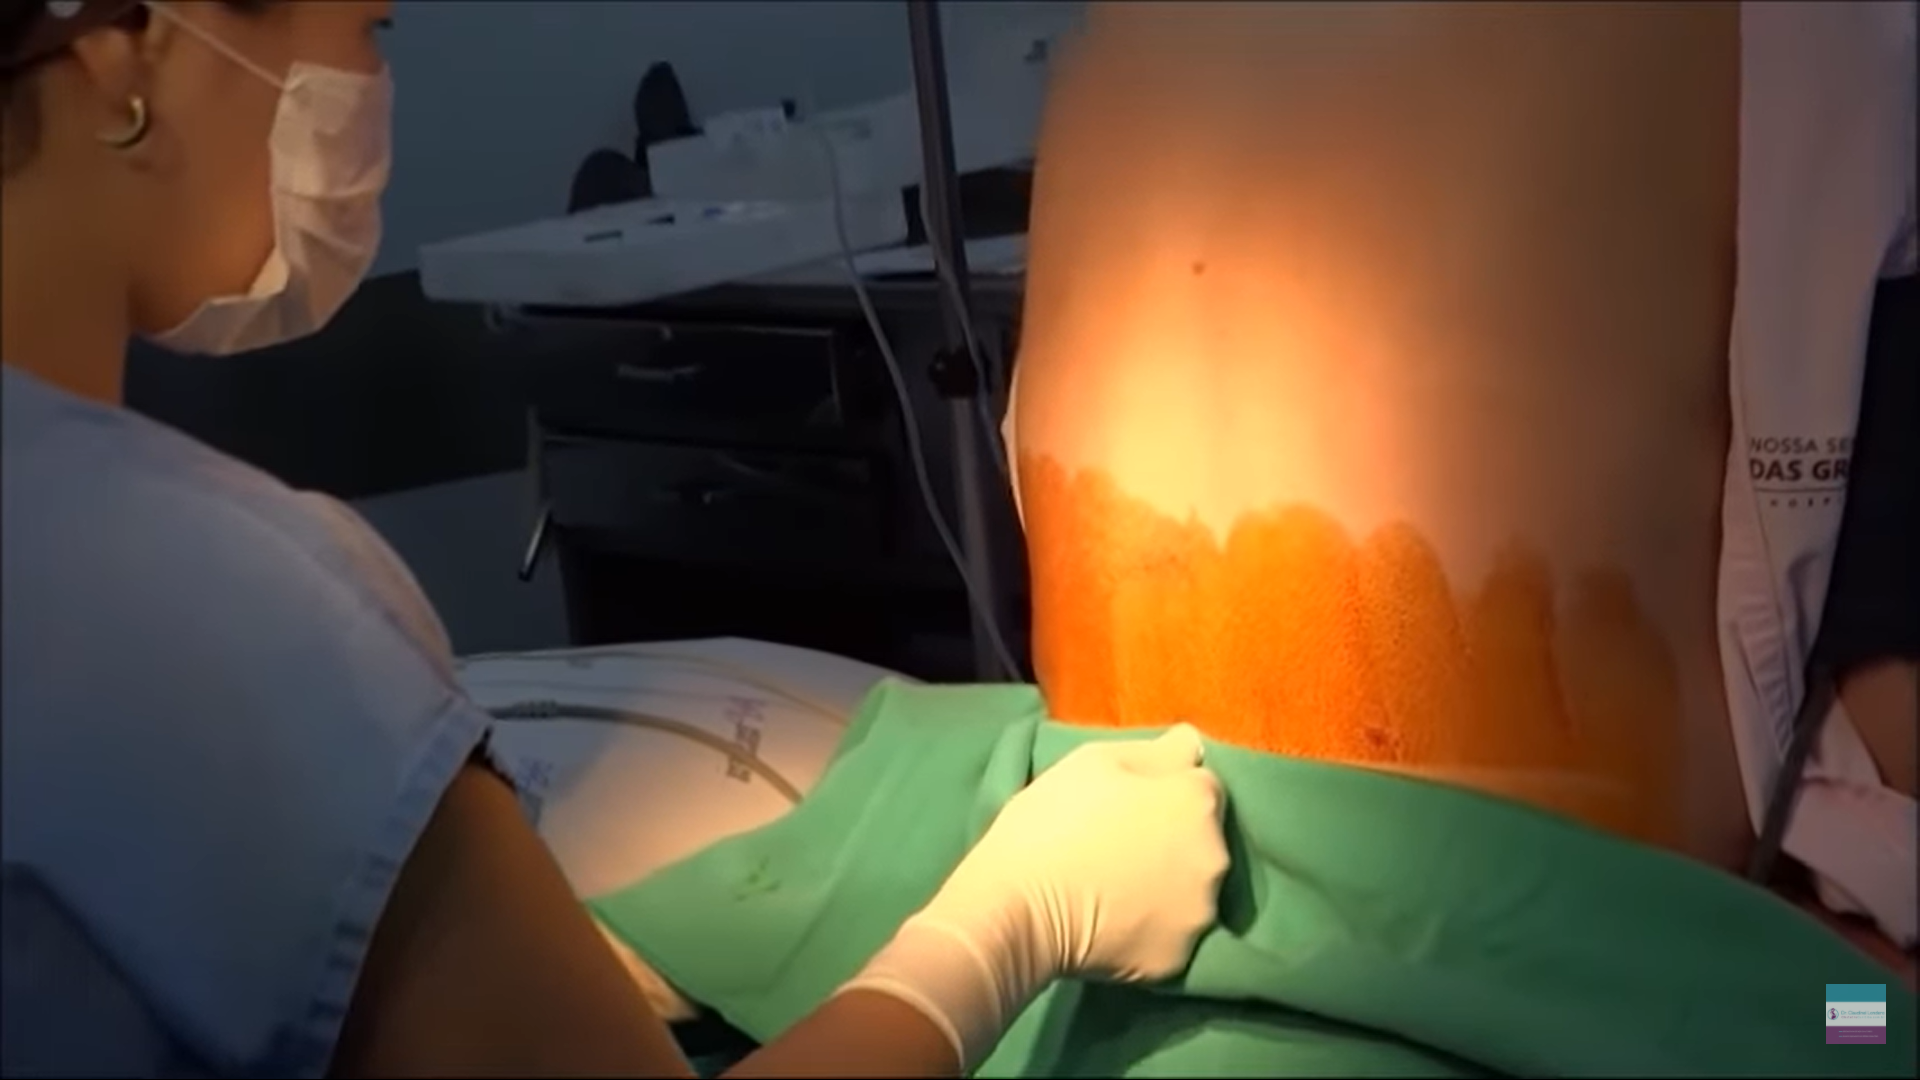
\includegraphics[width=0.6\linewidth]{capitulos/figuras/0.marcacaoPonto.png}
    \caption{Palpação para determinação do ponto de inserção da agulha \cite{Londero2018}.}
    \label{fig:marcacaoPonto}
\end{figure}

\begin{figure}[ht!]
    \centering
    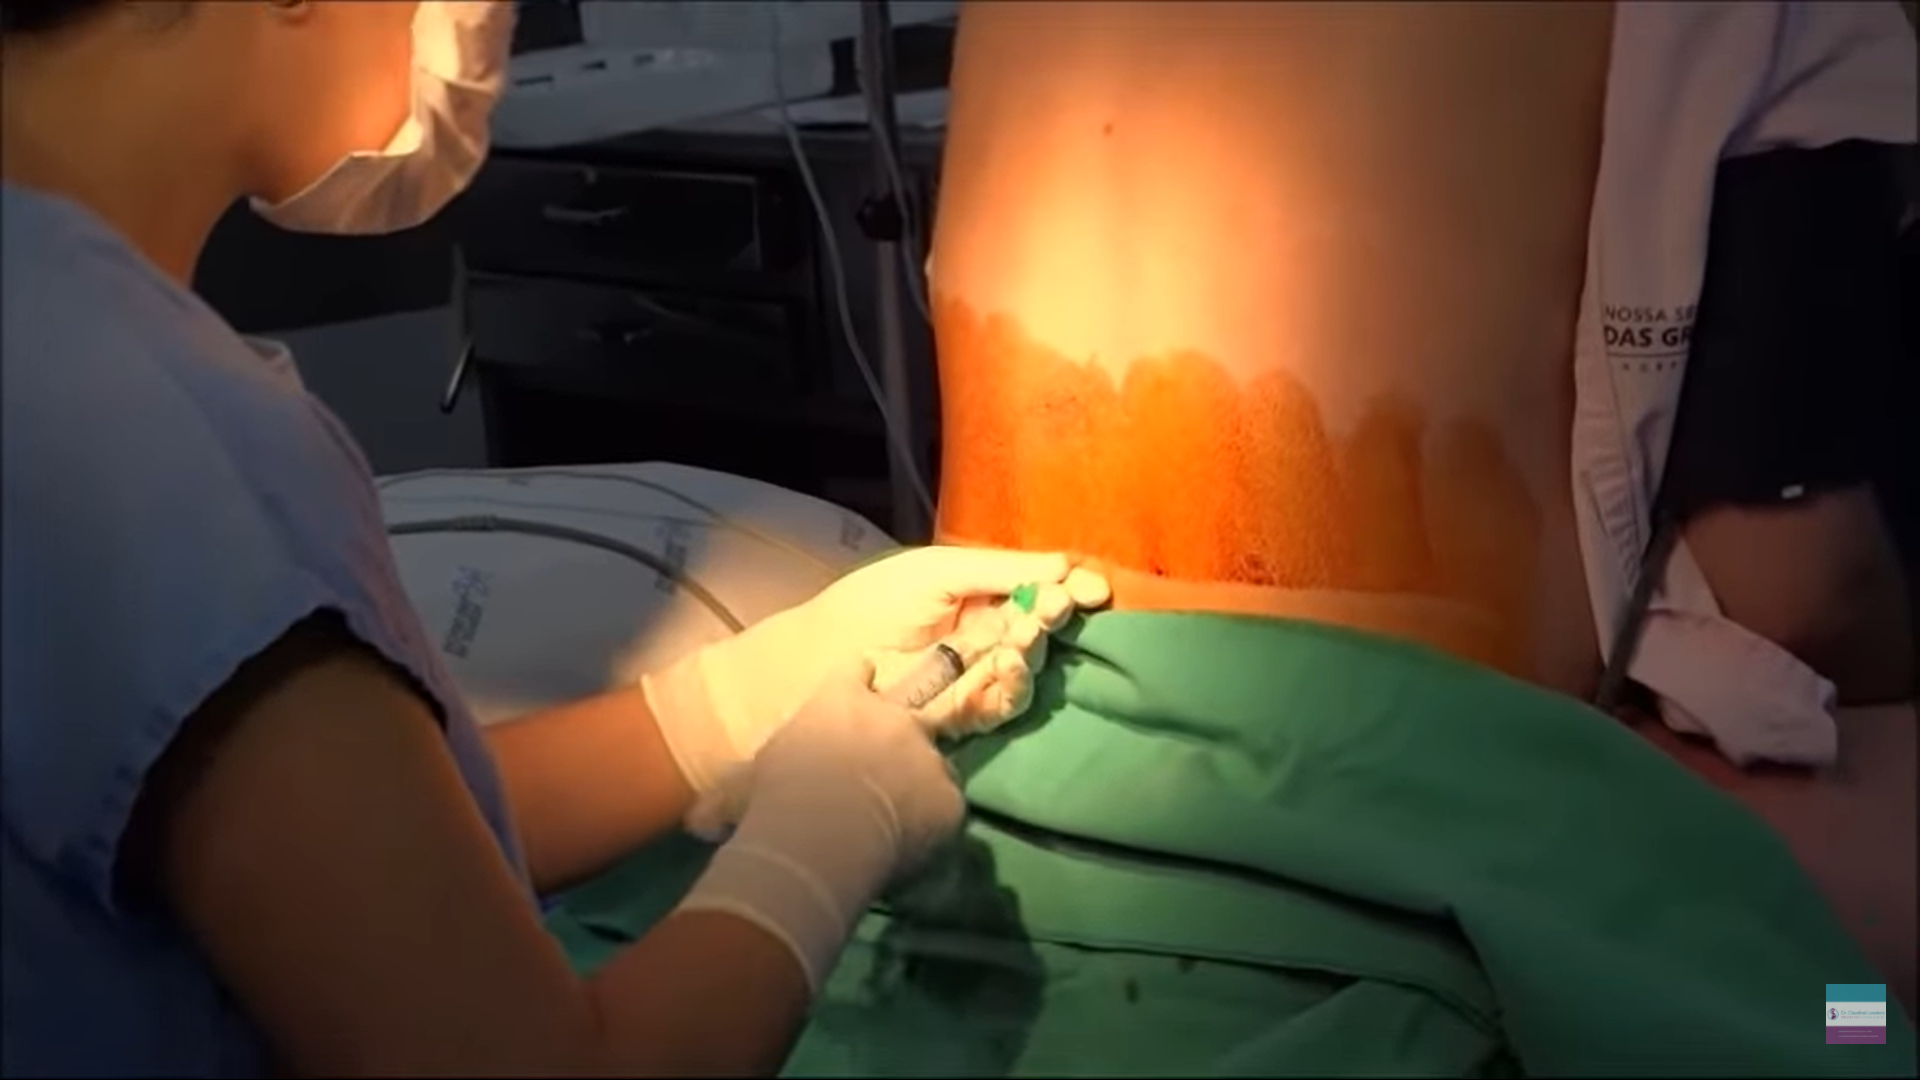
\includegraphics[width=0.6\linewidth]{capitulos/figuras/1.AnestesiaLocal.png}
    \caption{Aplicação da anestesia local \cite{Londero2018}.}
    \label{fig:anestesiaLocal}
\end{figure}

Existem duas principais abordagens de inserção da agulha para efetuação das anestesias regionais. Estas são denominadas mediana (\textit{midline}) e paramediana (\textit{paramedian}). A abordagem mediana é tida como a mais tradicional e, portanto  utilizada com mais frequência. No estudo de \textcite{Wantman2006} conduzido no Reino Unido esta foi a abordagem escolhida por 96\% dos anestesistas. Um dos motivos para o maior uso da abordagem mediana é a ausência de vasos sanguíneos no caminho da agulha nesta abordagem \cite{Bapat2015}. A abordagem paramediana é mais recomendada para pacientes idosos \cite{Ahsan-ul-Haq2005} devido à modificação degenerativa da coluna vertebral \cite{Boon2003} e calcificação dos ligamentos interespinhoso e supra-espinhoso \cite{Wantman2006}. A abordagem paramediana também pode ser mais viável que a mediana em pacientes obesos pela dificuldade na identificação da crista ilíaca nestes pacientes. Isto por que a camada de gordura faz com que a linha média seja mais difícil de localizar através da apalpação do médico \cite{N.2013}. Na abordagem mediana a agulha é inserida na linha média da coluna vertebral sendo feita sobre o plano sagital que pode ser observado na Figura~\ref{fig:planosAnatomicos}. Na paramediana existe certa angulação lateral entre a linha da coluna e a inserção da agulha é feita portanto uma movimentação da agulha no plano axial. As duas abordagens podem ser observadas no corte transversal da coluna na Figura~\ref{fig:abordagensInsercaoAgulha}. 

\begin{figure}[ht!]
    \centering
    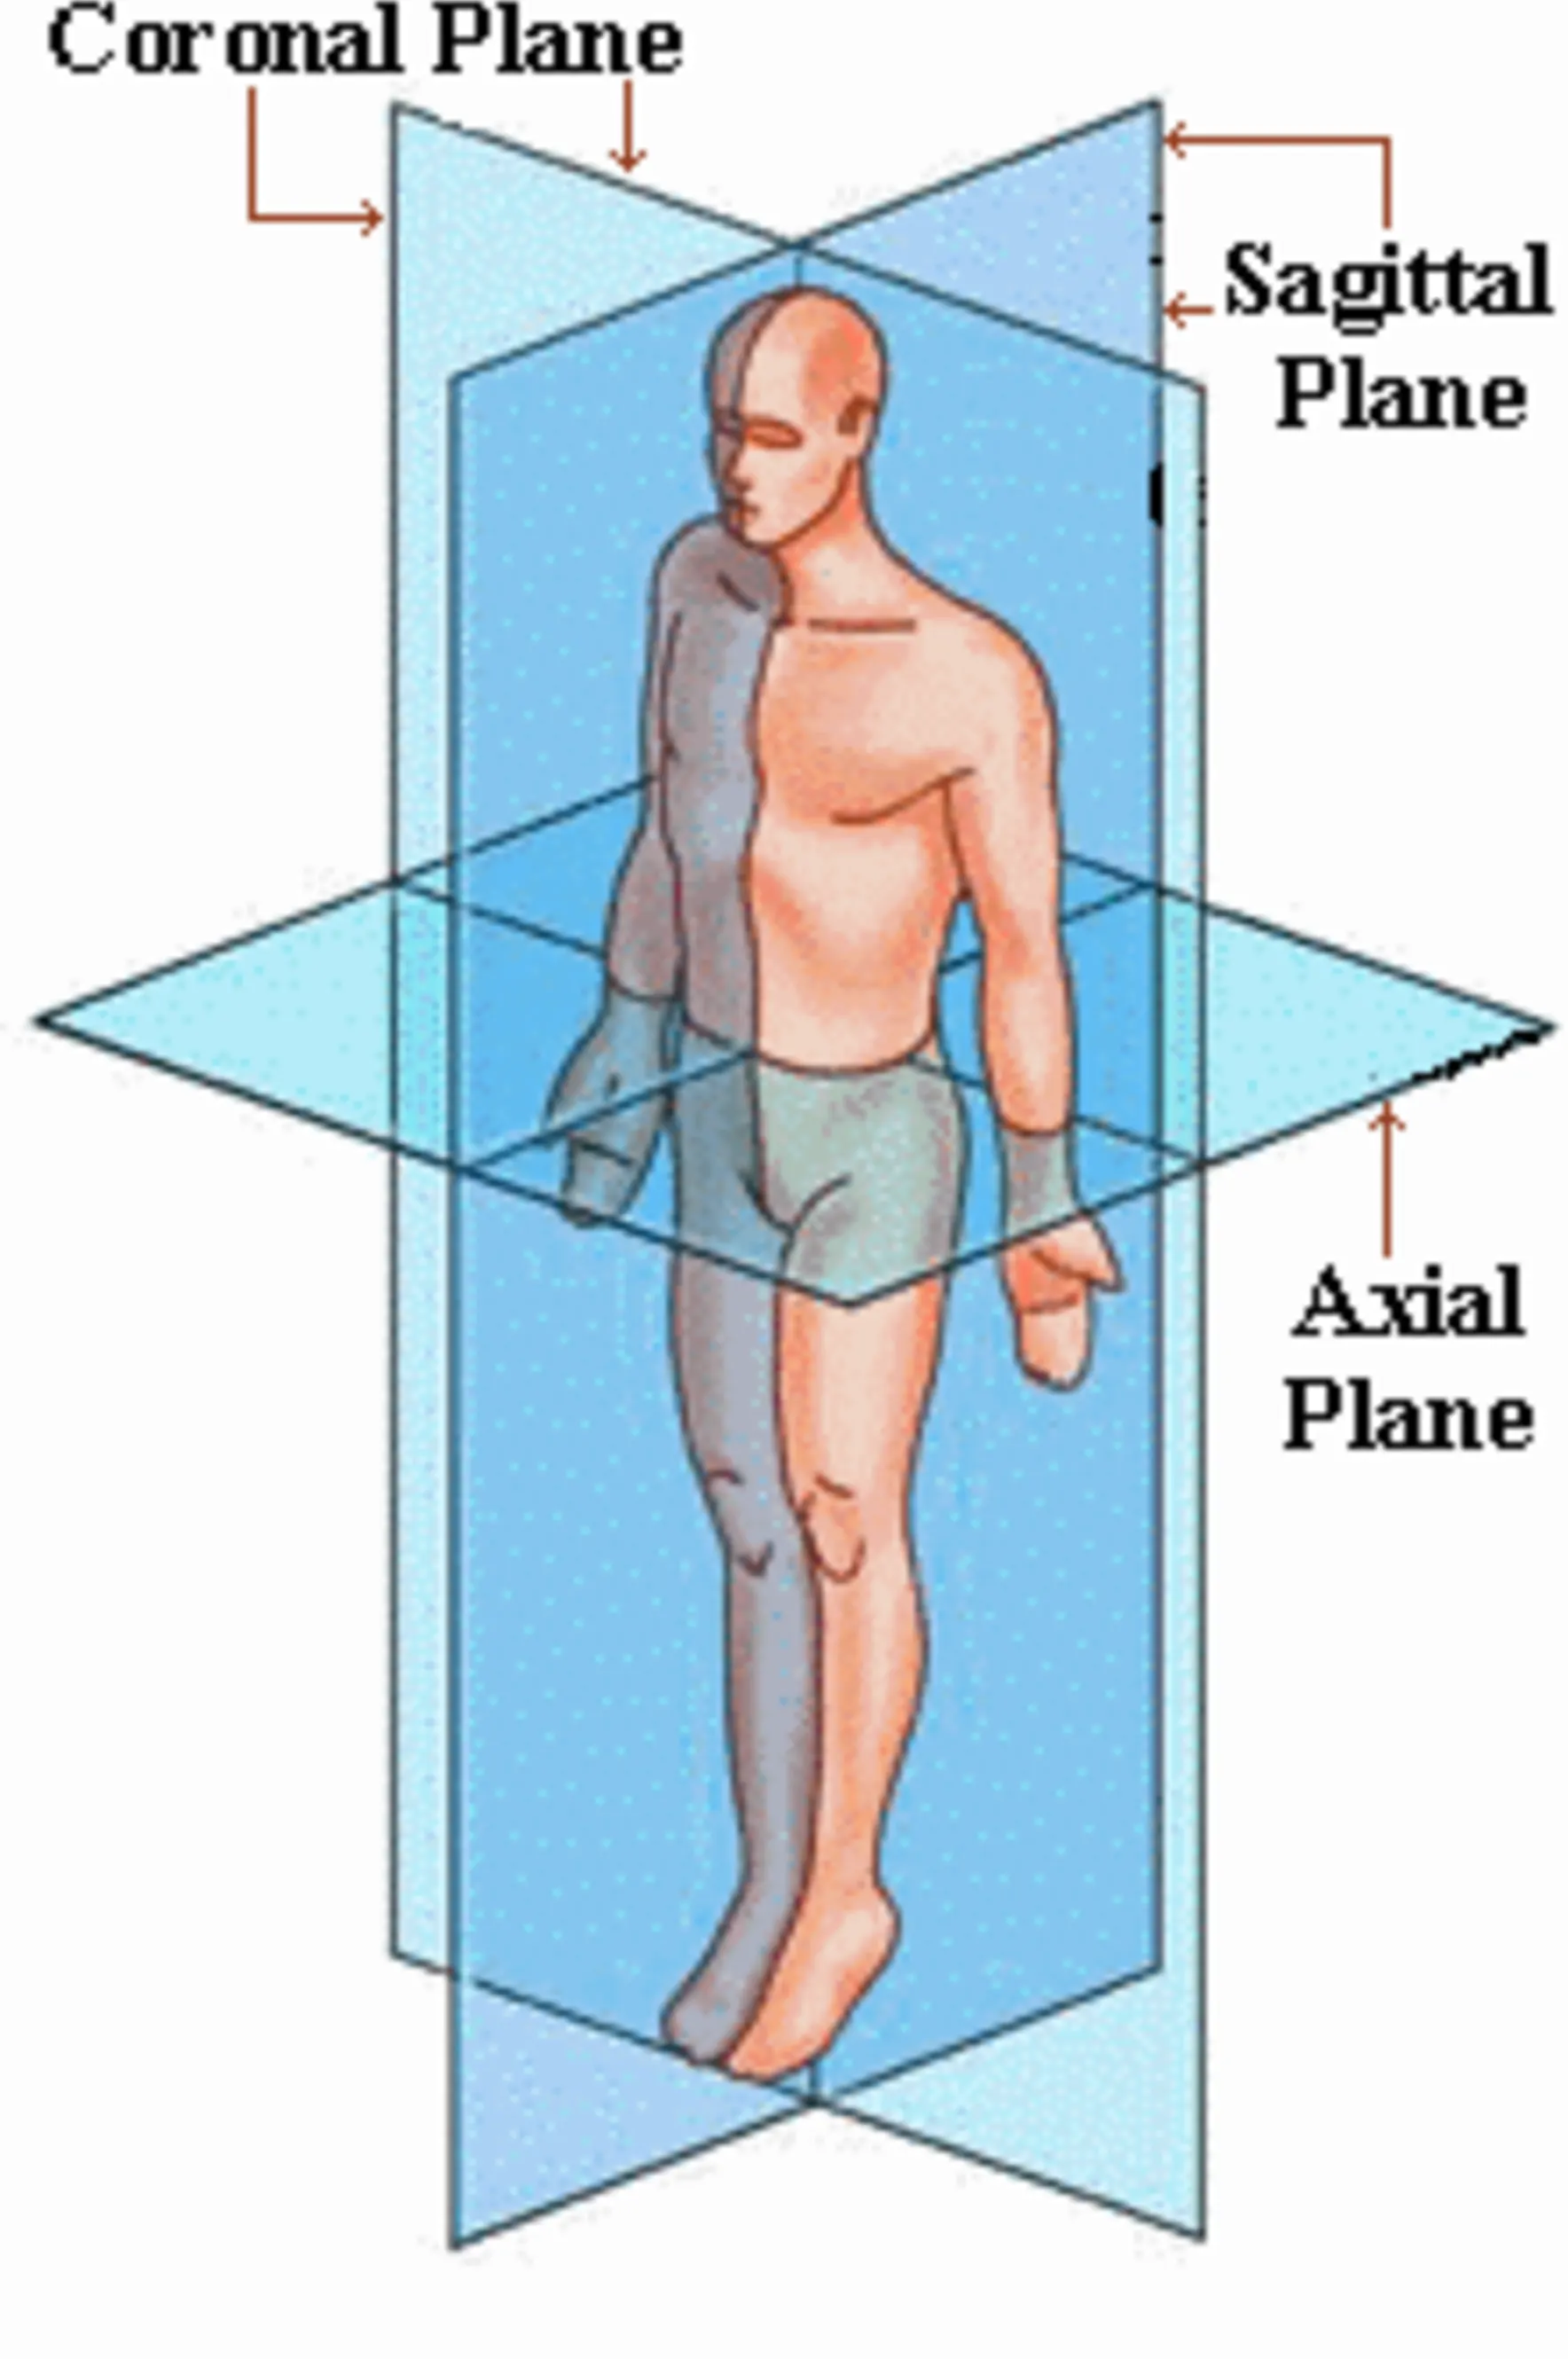
\includegraphics[width=0.35\linewidth]{capitulos/figuras/anatomical-planes.png}
    \caption{Representação dos planos anatômicos \cite{Bridwell2019}.}
    \label{fig:planosAnatomicos}
\end{figure}

\begin{figure}[ht!]
    \centering
    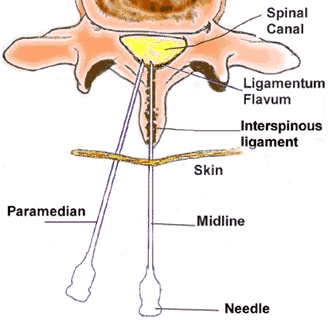
\includegraphics[width=0.6\linewidth]{capitulos/figuras/paramedian-midline-MedBroadcast-Tiff.png}
    \caption{Ilustração da abordagem mediana e paramediana para inserção de agulha \cite{MedBroadcast2018}.}
    \label{fig:abordagensInsercaoAgulha}
\end{figure}

\subsection{Anestesia Raquidiana} 
\label{sec:anestesiaRaquidiana}

A anestesia raquidiana  ou raqui, também chamada de bloqueio subaracnóideo ou  raquianestesia, é o nome dado quando a anestesia envolve a aplicação de um anestésico local no interior do espaço subaracnóideo. A posição ideal para a realização desta anestesia deve posicionar o paciente com a coluna lombar de modo que as vértebras fiquem fletidas para frente. É muito importante que seja feito um movimento na coluna de flexão criando uma convexidade para trás \cite{Anesclin2019}.

Existem duas principais formas para executar a raqui. Na primeira o paciente fica deitado de lado com as pernas dobradas, joelhos no abdômen e cabeça flexionada até que o queixo encoste no peito. Na segunda, o paciente fica sentado com as mãos nos joelhos, ombros relaxados e queixo no peito \cite{Anesclin2019}.

Neste tipo de anestesia, uma agulha de pequeno calibre é inserida nas costas do paciente até atingir o espaço subaracnóideo (localizado após a dura-máter), dentro da coluna espinhal. Em seguida, um anestésico é injetado dentro do líquido cérebro espinhal (\textit{líquor}), produzindo dormência temporária e relaxamento muscular (Figura~\ref{fig:injecaoAnestesico}). Anestesias raquidianas são aplicadas de forma mais frequente em espaços intervertebrais abaixo da segunda vértebra lombar (L2) e acima da quinta (L5), normalmente entre a L3 e L4 \cite{Wikipedia2019, Londero2018}. A Figura~\ref{fig:camadasPuncaoLombar} ilustra em um corte sagital da coluna as diferentes camadas que são cruzadas por uma agulha durante o procedimento de punção lombar até chegar ao espaço subaracnóideo. Considerando as duas abordagens de inserção da agulha (mediana e paramediana) as camadas onde a agulha pode passar desde a pele até o espaço subaracnóideo são: gordura subcutânea, músculo, ligamento supraespinhoso, ligamento interespinhoso, ligamento amarelo (\textit{flavum}), espaço epidural e dura-máter. O processo espinhoso que também aparece entre a pele e o espaço subaracnóideo na Figura~\ref{fig:camadasPuncaoLombar} não foi listado, pois, por ser uma camada de osso, ela não é perfurada pela agulha e sim uma camada intransponível em relação ao processo de punção. A abordagem paramediana evita a passagem pelos ligamentos supraespinhoso e interespinhoso fazendo com que após a camada de músculo se atinga diretamente o ligamento amarelo. Já na abordagem mediana usualmente não se passa pela camada de músculo.

\begin{figure}[ht!]
    \centering
    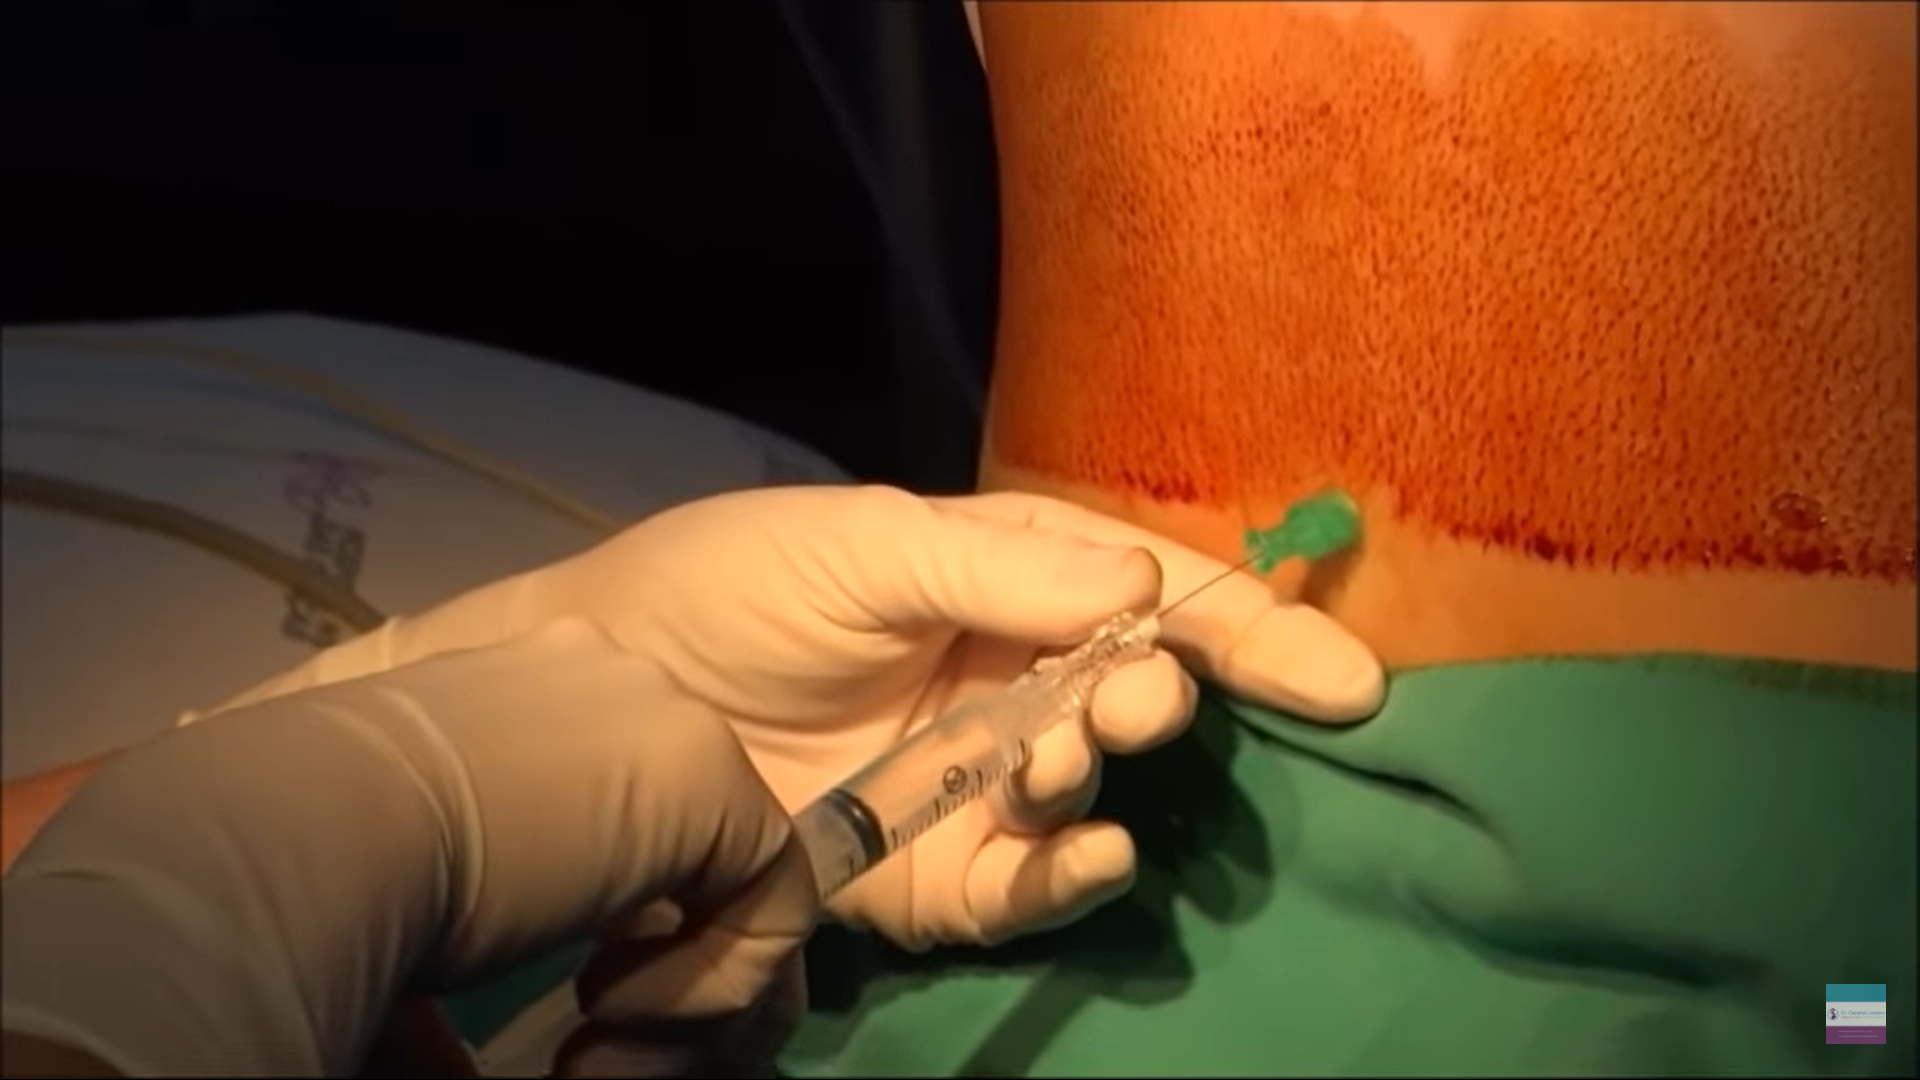
\includegraphics[width=0.6\linewidth]{capitulos/figuras/4.InjecaoAnestesico.png}
    \caption{Injeção do liquido anestésico no espaço subaracnóideo  \cite{Londero2018}.}
    \label{fig:injecaoAnestesico}
\end{figure}

\begin{figure}[ht!]
    \centering
    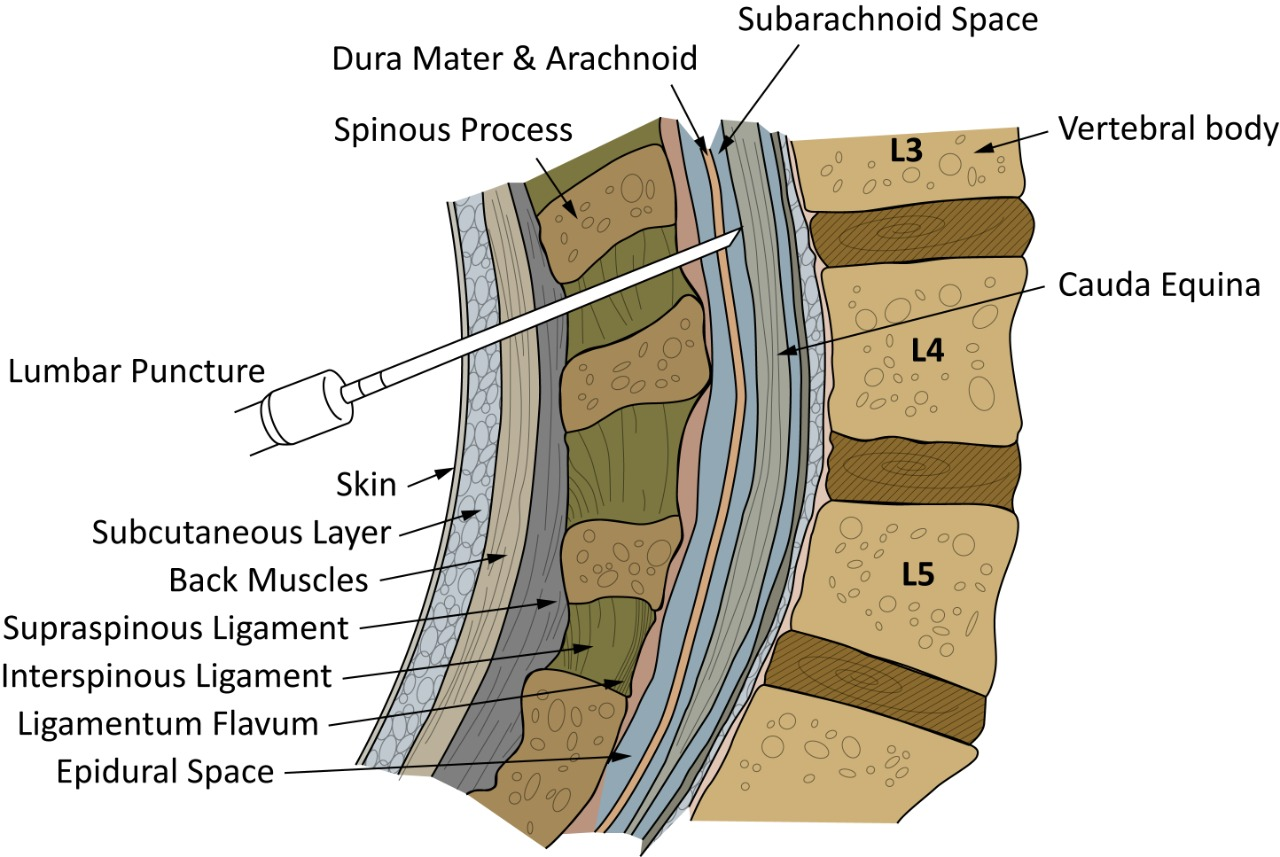
\includegraphics[width=0.6\linewidth]{capitulos/figuras/lumbar.puncture.tisssues.jpeg}
    \caption{Camadas cruzadas pela agulha numa punção lombar.}
    \label{fig:camadasPuncaoLombar}
\end{figure}

A ação do anestésico dentro da coluna espinhal é a de bloquear os nervos que passam pela coluna lombar, fazendo com que os estímulos dolorosos vindos de membros inferiores e do abdômen não cheguem ao cérebro. A raquianestesia é muito usada para procedimentos ortopédicos de membros inferiores assim como na região abdominal e cirurgias obstétricas de parto normal e cesarianas \cite{Pinheiro2018}.

A grande vantagem da anestesia raquidiana em relação a peridural é que nesta é necessário o uso de uma pequena quantidade de anestésico local. Esta característica reduz consideravelmente o risco de intoxicação por meio do elemento anestésico. Por outro lado a maior desvantagem no uso deste tipo de anestesia está na dor de cabeça que os pacientes sentem após a perfuração da dura-máter. Este sintoma é causado pela lesão na dura-máter que pode permanecer aberta por alguns dias após o procedimento, provocando perda do \textit{líquor} do espaço subaracnóideo. Com o uso de agulhas de menor diâmetro a incidência desta dor de cabeça foi consideravelmente reduzida \cite{INFOESCOLA2018}. 

\section{Realidade Virtual}

A \acrlong{RV} está presente quando se usa a tecnologia para criar a ilusão de que se está em um ambiente que não está lá ou não existe. Ela é uma aproximação da realidade experimentada por nós através dos nossos sentidos e sistemas de percepção. A nossa percepção da realidade vem através dos nossos sentidos. Portanto, uma vez apresentando aos sentidos às informações esperadas, sendo estas reais ou não, a nossa percepção da realidade irá se guiar por estes estímulos. Os sentidos mais comuns são visão, olfato, paladar, audição e tato. Porém também possuímos outros sentidos que afetam as nossas percepções do mundo, como por exemplo: o senso de equilíbrio, o sentimento de forças, pesos e deslocamentos sentidos por nossos membros \cite{VRS2018}.

Atualmente, a chamada \acrfull{RV} utiliza um computador para criar um ambiente virtual tridimensional. A intenção é a de simular uma realidade apresentando os elementos desejáveis para os sentidos do usuário, visando cumprir um objetivo através da interação de um ou mais usuários com este ambiente. Estes usuários se tornam parte deste ambiente virtual, total ou parcialmente, podendo manipular objetos ou executar um conjunto de ações \cite{VRS2018}.

A \acrshort{RV} possui uma série de usos sociais como, por exemplo, o tratamento de fobias. Há trabalhos para aracnofobia \cite{Carlin1997}, para aicmofobia ou medo de agulhas \cite{Galoustian2018}, para aerofobia ou medo de voar \cite{Rothbaum2006}, para acrofobia ou medo de altura \cite{Edwards2018} ou de forma mais geral para o medo e a ansiedade \cite{Goldman2017}. A Figura~\ref{fig:medoAltura} ilustra a aplicação para tratamento da acrofobia. Em primeiro plano a usuária com os óculos de realidade virtual e no segundo plano o ambiente virtual simulando ambientes de escadas e plataformas com fundo transparente.

\begin{figure}[ht!]
    \centering
    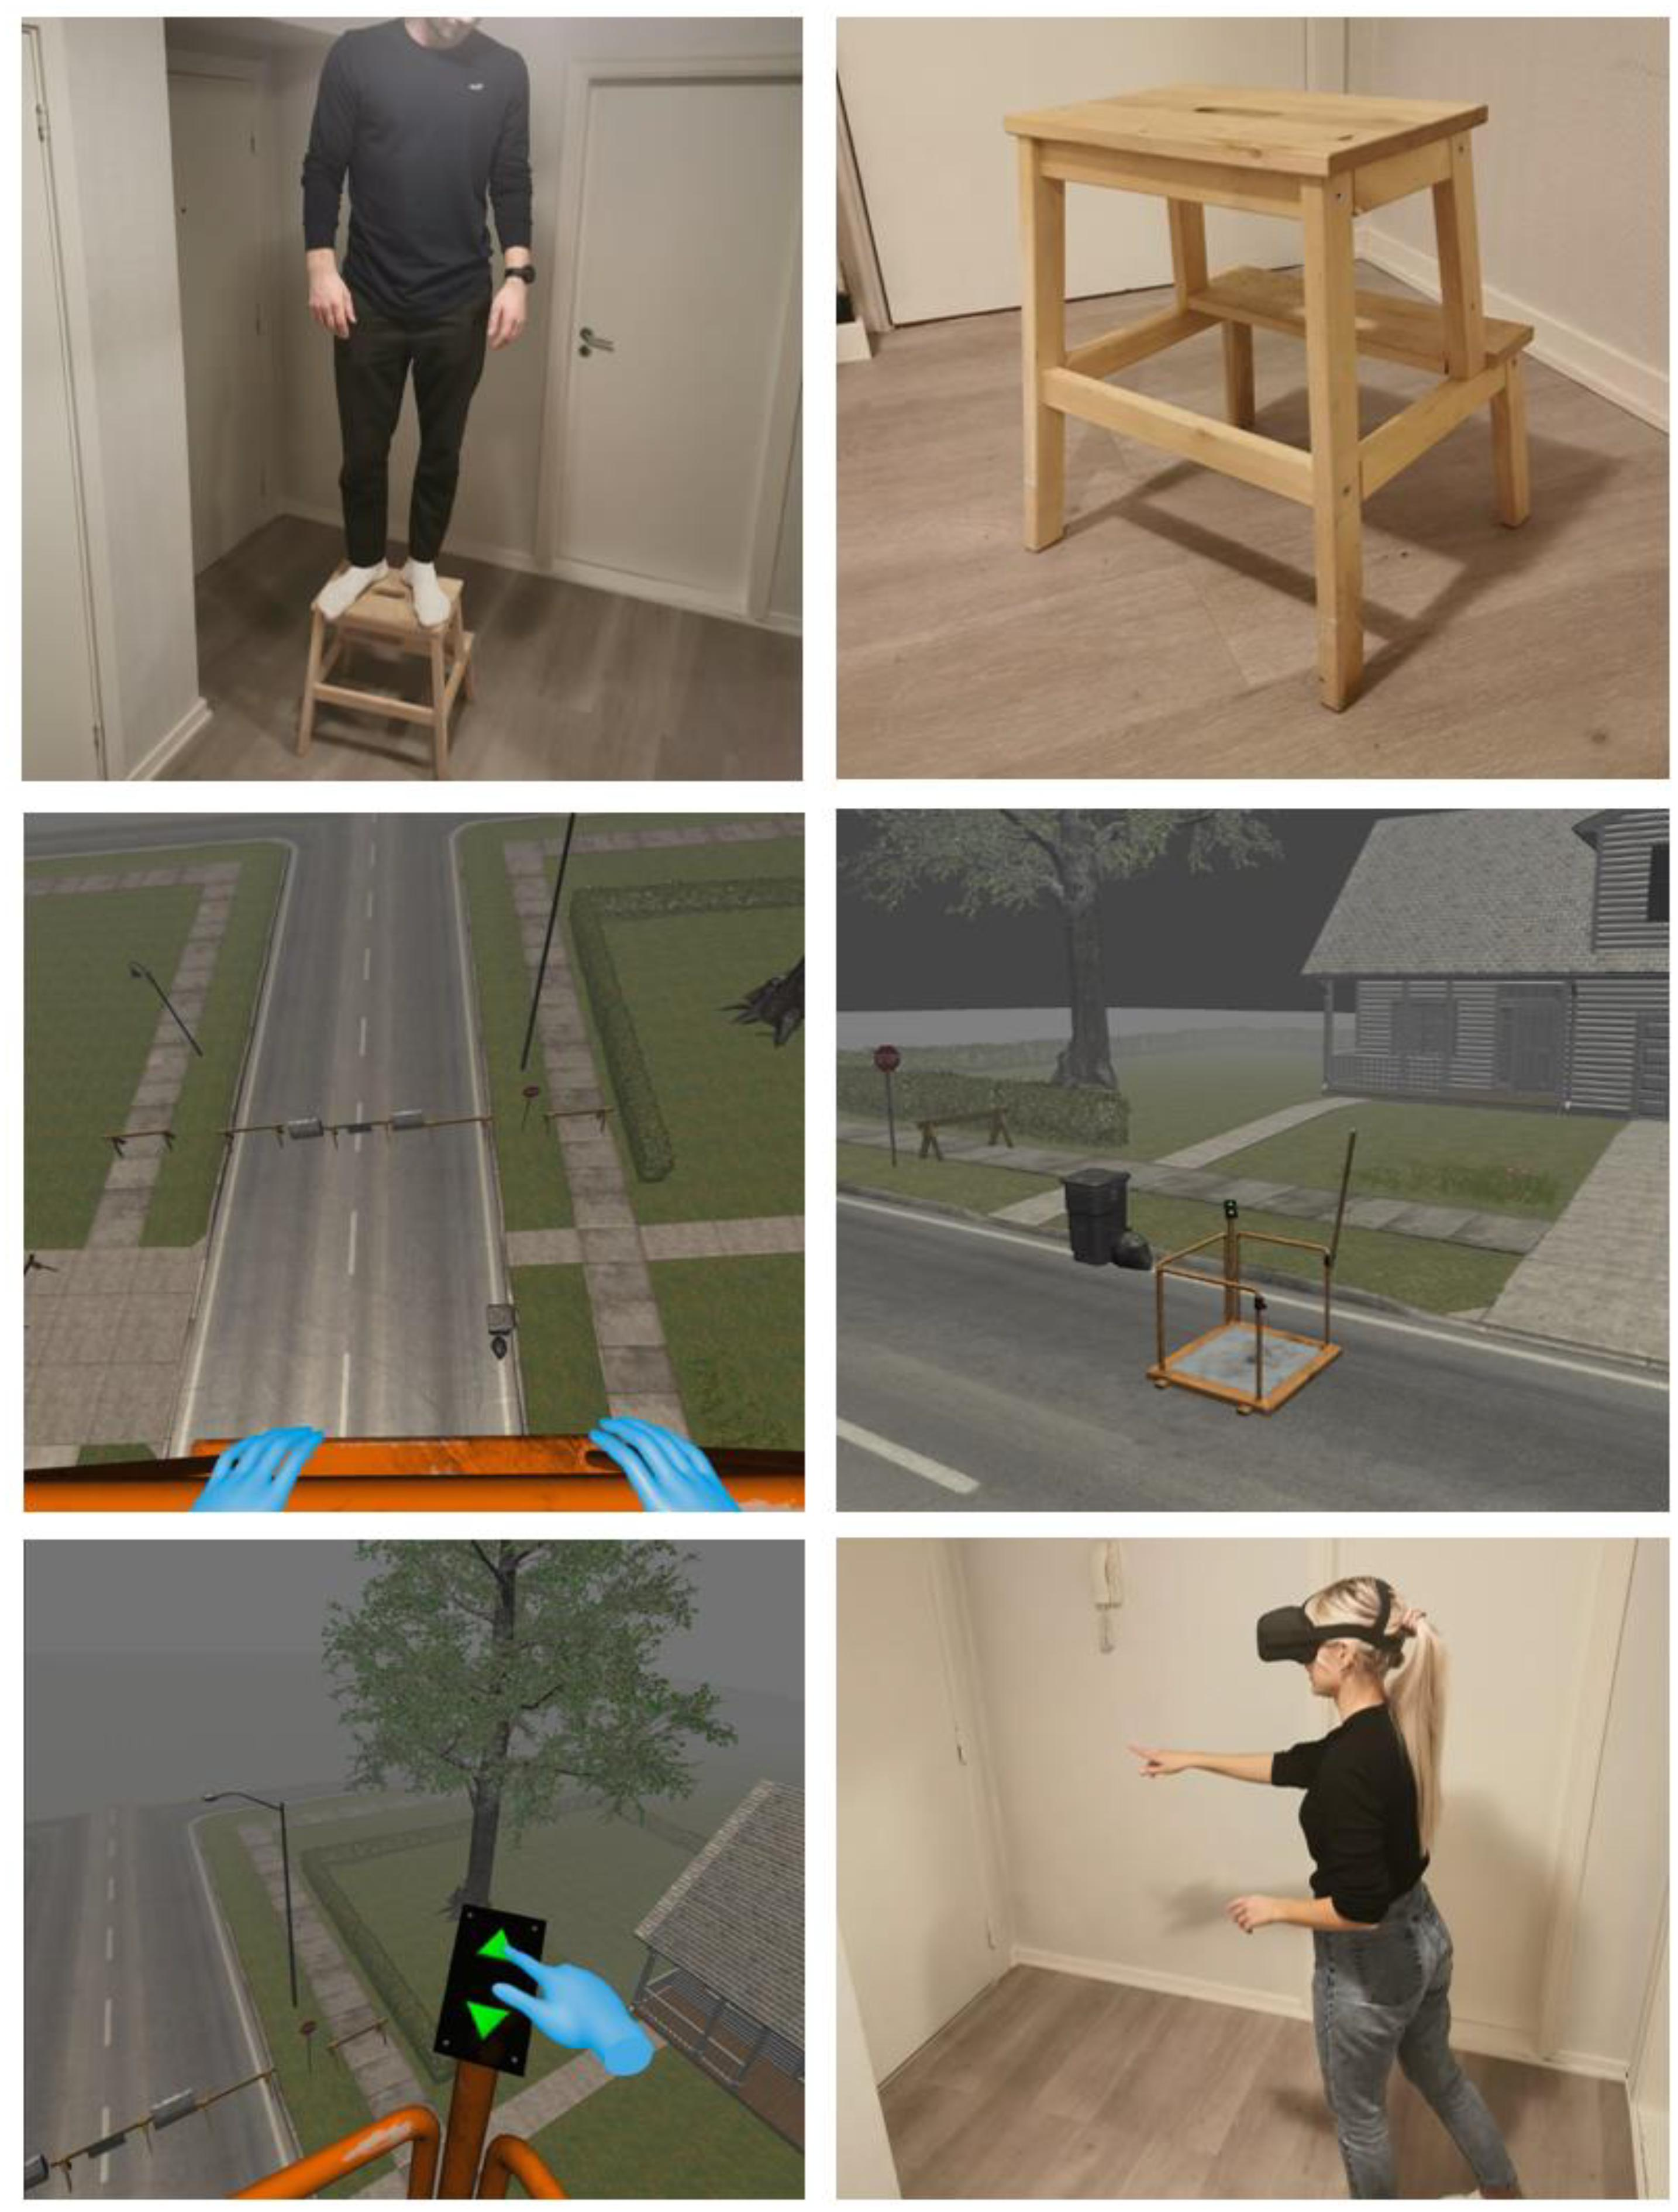
\includegraphics[width=0.6\linewidth]{capitulos/figuras/fear_of_heights.jpg}
    \caption{Exemplo de aplicação que usa \acrshort{RV} no tratamento da acrofobia \cite{Edwards2018}.}
    \label{fig:medoAltura}
\end{figure}

A indústria do entretenimento através de filmes e jogos provocou uma grande evolução de técnicas de \acrshort{RV} que posteriormente foram aplicadas em áreas mais “sérias” como o desenvolvimento pessoal e treinamento \cite{Ma2011, Prensky2001, Smith2011}. Na prática a \acrshort{RV} deve ser considerada como uma possibilidade sempre que o que se deseja fazer é muito perigoso, caro ou impraticável de ser realizado concretamente. Por conta destas características ela é muito usada nas áreas da educação, da saúde e militar \cite{VRS2018}. Conforme a tecnologia que permite a criação e simulação de ambientes virtuais se torna mais barata, mais aplicações são criadas com o uso destas ferramentas.

\section{Dispositivos Hápticos}

O termo \textit{haptics} é usado para descrever a ciência que estuda e simula a pressão, textura, vibração e outras sensações biológicas relacionadas ao toque. A sensação do toque se origina em estímulos mecânicos, elétricos, térmicos ou químicos na pele \cite{Burdea1996}. O tato não está localizado numa região específica do corpo como os demais sentidos. Ele está distribuído por todo o corpo através do órgão sensorial do toque, nossa pele, articulações, músculos e tendões. O senso do toque se divide em duas sensações: cinética e tátil. Forças e torques são sensações cinéticas que sentimos nos músculos, tendões e articulações. Já as sensações táteis como pressão, deformação e vibração são sentidas por mecano receptores que possuímos na nossa pele \cite{Culbertson2018}. 

Os primeiros dispositivos hápticos foram originados dos braços robóticos usados para o controle remoto de robôs \cite{Zurawski2005} As aplicações de tecnologias hápticas são muito variadas envolvendo, por exemplo, projetos de engenharia e aplicações de manufatura \cite{Sharma2001}, entretenimento (videogames e filmes), celulares, relógios inteligentes e até mesmo a indústria automobilística \cite{Smith2019}. Estes dispositivos possuem elementos mecânicos de entrada e saída para interação com o usuário. Uma ou mais partes do dispositivo em contato com o usuário são monitorados no espaço físico e o dispositivo oferece como retorno força e torque. Desta forma um canal bidirecional de interação entre o ambiente virtual e o usuário é criado \cite{Coles2011}. Estes dispositivos estão sendo cada vez mais utilizados hoje em dia tanto pela evolução da sua tecnologia como pela diminuição dos preços. Com o avanço da tecnologia estes dispositivos estão se tornando cada vez mais flexíveis representando mais fielmente os movimentos. Isto ocorre  através do uso de conceitos de restrição parcial a movimentos, deslocamentos e da inclusão de mais graus de liberdade, \textit{\acrfull{DoF}}. 

O número de graus de liberdade de um dispositivo háptico se refere ao número de maneiras diferentes em que este pode se mover ou criar forças. Como exemplo, dispositivos com 3 graus de liberdade podem rastrear posições e criar forças ao serem movidos nas direções: direita-esquerda, frente-trás e cima-baixo \cite{HAPTICSHOUSE2019}. O principal objetivo no uso destes dispositivos é o aumento da sensação de imersão em um ambiente de realidade virtual. 

Em relação à área médica, os dispositivos hápticos vem sendo utilizados na maioria dos trabalhos de simulação de procedimentos médicos \cite{Coles2011,Escobar-Castillejos2016}. Eles são usados para simular o uso de ferramentas em cirurgias e ajudaram a impulsionar o sucesso das práticas em simuladores virtuais. Isto aconteceu ao proporcionar o controle dos graus de liberdade de deslocamentos, a restrição aos movimentos e as respostas às atitudes do usuário como forças de reação ou \textit{feedback} \cite{Gerovich2004}. Estes dispositivos eletromecânicos existem nas mais diversas formas e são adaptados para uma grande variedade de procedimentos médicos como, por exemplo, no treinamento de laparoscopia \cite{Srinivasan2004}, biopsia de próstata \cite{Sclaverano2009}, cirurgia de fígado \cite{Mastmeyer2016}, exames de mama \cite{Brazil2017,Jeon2010,Ribeiro2014,Solanki2010}, simulação de apalpação \cite{Ribeiro2016} e punções epidurais \cite{N.2013, Brazil2018}. Alguns sistemas usam mais de um háptico como em punções de agulha guiadas por ultrassom que usam um equipamento para simular a agulha e outro para o ultrassom \cite{Ni2011,Vidal2008}. Outros chegam a fazer o uso de três dispositivos como o PalpSim de forma a simular o toque das mãos do usuário num paciente virtual \cite{Coles2011b}. 

\textcite{Culbertson2018} identificaram como 3 as principais categorias de sistemas hápticos: compreensíveis, vestíveis e palpáveis. Um exemplo visual destes tipos pode ser visto na Figura~\ref{fig:tiposHapticos}. Os sistemas compreensíveis são dispositivos tipicamente cinéticos (\textit{feedback} de força) que normalmente possuem uma base fixa e permitem ao usuário empurrar e ser empurrado de volta. Sistemas vestíveis são tipicamente táteis montados nas mãos ou em outras partes do corpo e provocam sensações diretamente na pele. Os sistemas palpáveis são dispositivos de encontro que permitem ao usuário explorar toda a superfície \cite{Culbertson2018}. Os dispositivos a serem explorados aqui são os de sistemas compreensíveis. Estes foram os tipos de hápticos utilizados nos simuladores computacionais relacionados ao tema desta tese estudados e citados na seção~\ref{sec:simuladoresComputacionais}. \textcite{Ribeiro2016} fizeram uma revisão sobre dispositivos usados na simulação de procedimentos que envolvem o toque da mão do médico para identificação de características e anormalidades sob a pele. Os autores analisaram 57 trabalhos e mais da metade fez uso dos dispositivos da família \textit{Phantom}. Os dispositivos desta família serão listados nesta seção.

\begin{figure}[ht!]
    \centering
    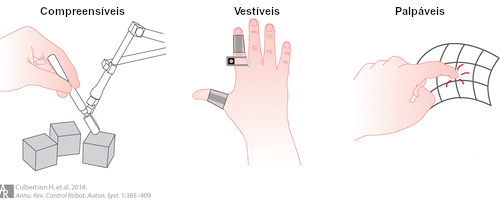
\includegraphics[width=0.8\linewidth]{capitulos/figuras/tipos.hapticos-portugues.png}
    \caption{Tipos de sistemas háptico \cite{Culbertson2018}.}
    \label{fig:tiposHapticos}
\end{figure}

Nas figuras~\ref{fig:hapticoNovintFalcon}, \ref{fig:hapticoTouch}, \ref{fig:hapticoTouchX} e  \ref{fig:hapticoPremium}, os dispositivos aparecem representados ordenados pelas suas complexidades i.e. dos mais simples (mais antigos e com menos recursos) aos mais avançados (mais novos). Todos estes dispositivos são exemplos de sistemas tipicamente cinéticos. Os mais novos possibilitam maior número de graus de liberdade para os movimentos assim como possibilitam mais forças e momentos de reação. O Novint Falcon ® (Figura~\ref{fig:hapticoNovintFalcon}), lançado em 2007, tem como interface com o usuário uma esfera onde o usuário deve colocar os dedos da mão para fazer os movimentos no caso do seu uso mais comum. No que diz respeito à liberdade de movimento este mecanismo proporciona uma interação 3D com o computador no lugar da interação 2D proporcionada pelo mouse. Ele possui 3 graus de liberdade de movimento e de forças. Nesta esfera existem quatro botões para interação e existem sensores para determinar a posição do cursor e motores para controlar as forças a serem transmitidas para o usuário. Existem versões onde a esfera é substituída, por exemplo, por um dispositivo semelhante a uma pistola para que o dispositivo seja usado em jogos de tiros de primeira pessoa \cite{VRS2017}. 

\begin{figure}[ht!]
    \centering
    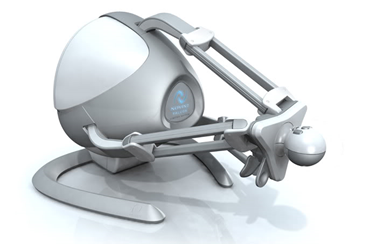
\includegraphics[width=0.4\linewidth]{capitulos/figuras/hapticoNovintFalcon.png}
    \caption{Dispositivo háptico Novint Falcon ® \cite{HAPTICSHOUSE2019}
    \label{fig:hapticoNovintFalcon}.}
\end{figure}

\begin{figure}[ht!]
    \centering
    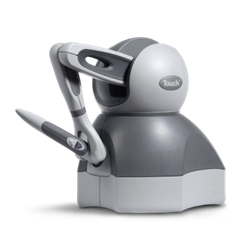
\includegraphics[width=0.4\linewidth]{capitulos/figuras/hapticoTouch.png}
    \caption{Dispositivo háptico Geomagic Touch ® / Phantom Omni ® \cite{3DSystems2018}.}
    \label{fig:hapticoTouch}
\end{figure}

\begin{figure}[ht!]
    \centering
    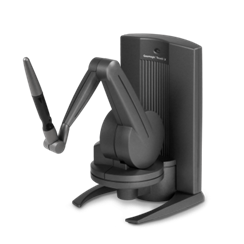
\includegraphics[width=0.4\linewidth]{capitulos/figuras/hapticoTouchX.png}
    \caption{Dispositivo háptico Geomagic Touch X ® / Phantom Desktop ® \cite{3DSystems2018}.}
    \label{fig:hapticoTouchX}
\end{figure}


\begin{figure}[ht!]
    \centering
    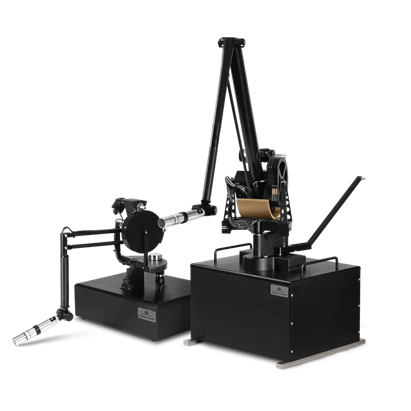
\includegraphics[width=0.4\linewidth]{capitulos/figuras/hapticoPhantomPremium.png}
    \caption{Dispositivo háptico Phantom Premium ® \cite{3DSystems2018}.}
    \label{fig:hapticoPremium}
\end{figure}

Os hápticos da família \textit{Phantom Geomagic Touch} ® (Figura~\ref{fig:hapticoTouch}) e \textit{Geomagic Touch} X ® (Figura~\ref{fig:hapticoTouchX}) apresentam uma peça que simula uma caneta para manipulação do usuário da mesma forma que a esfera no dispositivo da Figura~\ref{fig:hapticoNovintFalcon}. Nas canetas também existem botões para interação e da mesma forma estas também são substituíveis por partes com formas mais adequadas ao procedimento que estas pretendem simular. O dispositivo \textit{Geomagic Touch} X ® possui a mesma liberdade de movimento do \textit{Geomagic Touch} ®, porém possibilita \textit{feedback} de reações maiores. Ambos apresentam 6 graus de liberdade de movimento e 3 graus de liberdade no retorno de forças. Estes dispositivos, portanto mapeiam a posição 3D e orientação, mas somente apresentam \textit{feedback} de forças direcionais \cite{Forsslund2013}.

O \textit{Phantom Premium} ® (Figura~\ref{fig:hapticoPremium}) está disponível nas versões \textit{Premium} 1.0, \textit{Premium 1.5} e 1.5/HF, e \textit{Premium} 3.0. Estas evoluem não só o \textit{feedback} de reações como também os graus de liberdade dos movimentos. Enquanto o \textit{Phantom Premium} 1.0 ® simula o movimento do giro do pulso na mão o \textit{Phantom Premium} 3.0 ® possibilita uma amplitude que simula os graus de liberdade de movimento de todo o braço humano desde o ombro \cite{3DSystems2018}. Este dispositivo possui 6 graus de liberdade tanto para movimento como retorno de forças o que o torna simétrico no número de sensores e motores (atuadores). São computadas forças e torques tanto da posição como da orientação deste dispositivo. Esta característica tem uma forte influencia no alto custo associado a este tipo de dispositivo \cite{Forsslund2013}.

\section{Modelagem de tecidos}
\label{sec:modelagemTecidos}

Um dos passos necessários para construção de um ambiente virtual para treinamento de raquianestesia é a criação de pacientes virtuais. Um importante aspecto da modelagem destes pacientes é como eles aparecem na tela da aplicação. Outro aspecto importante na simulação é ter uma estimativa da espessura dos tecidos envolvidos nestes tipos de anestesia. Para isto é necessária à modelagem do tamanho de todas as camadas de tecido pelos quais as agulhas passam para execução destes procedimentos. Uma ilustração destes tecidos que vão desde a pele até o espaço subaracnóide (onde deve ser aplicada a anestesia) pode ser vista na Figura~\ref{fig:camadasPuncaoLombar}. Nesta seção são descritos trabalhos relacionados com a modelagem da distância entre a pele e a dura-máter que é a camada imediatamente anterior ao espaço subaracnóide.

\begin{table}[!ht]
\begin{center}
\caption{Variáveis e unidades de medida utilizadas no texto.}
\label{tab:variaveisUnidades}
\begin{tabular}{|p{0.53\linewidth}|p{0.25\linewidth}|p{0.13\linewidth}|}
\hline
\textbf{Váriavel (sigla) - fórmula} & \textbf{Unidade} & \textbf{Unidade abreviada}\\
\hline\hline
Massa (M) & quilogramas & kg \\
Altura (A) & metros & m \\
Idade (I) & anos & - \\
\acrfull{IMC} - M/A\textasciicircum{}2 & quilogramas/metros\textasciicircum{}2 & kg/m\textasciicircum{}2 \\
\acrfull{DEE} & centímetros & cm \\
\hline
\end{tabular}
\end{center}
\end{table}

Na Tabela~\ref{tab:variaveisUnidades} são listadas as varáveis de entrada e saída dos métodos estudados nesta seção. Esta tabela exibe também as unidades destas variáveis que serão utilizadas em todo este trabalho.

Muitos trabalhos buscam relacionar a \acrfull{DEE} com as demais variáveis da Tabela~\ref{tab:variaveisUnidades}. A grande maioria dos trabalhos indica uma forte relação da \acrshort{DEE} com o \acrshort{IMC} \cite{Adegboye2017, Galbraith2018}. Estes dois trabalhos não fazem separação dos grupos populacionais por idade, sexo ou etnia, e usaram populações respectivamente de n=120 e n=317 pessoas entre homens e mulheres.

Os trabalhos citados a seguir analisaram somente ou de forma separada grupos de mulheres grávidas. Como este é o foco deste trabalho só serão comentadas aqui as conclusões referentes a estes grupos. Todos os trabalhos a seguir encontraram influencia do \acrshort{IMC} na determinação da \acrshort{DEE}, mas além desta relação também foram encontradas outras combinações em cada trabalho. O grupo étnico/populacional do individuo foi observado em conjunto com o \acrshort{IMC} em \cite{Sharma2011} estudo feito no \acrfull{RU}. A idade foi observada em conjunto com o \acrshort{IMC} num estudo em pacientes americanas em Michigan, EUA \cite{Clinkscales2007}. A altura, massa, idade e \acrshort{IMC} foram observados como relevantes em um estudo em pacientes da Índia \cite{Hazarika2016}. Estes dois últimos trabalhos construíram equações de regressão linear para determinação da \acrshort{DEE} para grupos de parturientes conforme pode ser visto na Tabela~\ref{tab:equacoesEstimativaDEE}.

\begin{table}[!ht]
\begin{center}
\caption{Equações para estimativa da DEE em grávidas.}
\label{tab:equacoesEstimativaDEE}
\begin{tabular}{|p{0.27\linewidth}|p{0.55\linewidth}|p{0.105\linewidth}|}
\hline
\textbf{Trabalho} & \textbf{Equação} & \textbf{Local da amostra}\\
\hline\hline
\cite{Clinkscales2007} & DEE = 3 + 0,11 IMC - 0,01 I & EUA \\
\cite{Hazarika2016} & DEE = 4,748 + 0,209 IMC + 4,703 A - 0,054 M & Índia \\
\hline
\end{tabular}
\end{center}
\end{table}

Os autores em \cite{Sharma2011} no lugar das equações apresentaram como resultado uma tabela com cinco pontos de cada par \acrshort{IMC} x \acrshort{DEE} para cada grupo populacional analisado. Estes dados podem ser vistos na Tabela~\ref{tab:DEEEstimadosSharma}. A definição dos grupos populacionais no estudo do \acrshort{RU} em \cite{Sharma2011} foi: Brancas (população do \acrlong{RU}, da Irlanda e qualquer outro grupo com cor de pele branca); Asiáticas ou Britânicas Asiáticas (população da Índia, Paquistão, Bangladesh ou qualquer outro grupo Asiático); Negras ou Britânicas negras (população de Africanas, Caribenhas ou outros grupos com cor da pele negra); e Chinesas e outros grupos étnicos (população da China, Japão, Malásia, Filipinas etc.). No grupo de nome Chinesas, além dos dados de pessoas desta origem moradoras do \acrshort{RU}, foram considerados dados de Chinesas (n=70) de um hospital de Singapura.

\begin{table}[!ht]
\begin{center}
\caption{\acrshort{DEE} estimados para os grupos populacionais de \cite{Sharma2011}.}
\label{tab:DEEEstimadosSharma}
\begin{tabular}{|l|llll|}
\hline
\multicolumn{1}{|c|}{\multirow{2}{*}{IMC (kg/m\textasciicircum{}2)}} & \multicolumn{4}{c|}{\acrshort{DEE} estimada (cm)}  \\ \cline{2-5} 
\multicolumn{1}{|c|}{} & \multicolumn{1}{c|}{Brancas} & \multicolumn{1}{c|}
{
\begin{tabular}[c]{@{}c@{}}Asiáticas/Britânicas \\ Asiáticas\end{tabular}} & \multicolumn{1}{c|}{\begin{tabular}[c]{@{}c@{}}Negras/Britânicas\\ Negras\end{tabular}} & \multicolumn{1}{c|}{Chinesas} \\ 
\hline\hline
20 & \multicolumn{1}{l|}{4,7} & \multicolumn{1}{l|}{4,5} & \multicolumn{1}{l|}{5,0} & 4,4\\ 
25 & \multicolumn{1}{l|}{5,3} & \multicolumn{1}{l|}{5,1} & \multicolumn{1}{l|}{5,7} & 4,7 \\ 
30 & \multicolumn{1}{l|}{6,0} & \multicolumn{1}{l|}{5,7} & \multicolumn{1}{l|}{6,5} & 5,1 \\ 
35 & \multicolumn{1}{l|}{6,6} & \multicolumn{1}{l|}{6,2} & \multicolumn{1}{l|}{7,2} & 5,4 \\ 
40 & \multicolumn{1}{l|}{7,2} & \multicolumn{1}{l|}{6,8} & \multicolumn{1}{l|}{8,0} & 5,7 \\ 
\hline
\end{tabular}
\end{center}
\end{table}

Na Tabela ~\ref{tab:PopulacaoPorEstudo} é apresentado o tamanho da população utilizada nestes estudos e as identificações da origem dos dados do estudo, isto é, os grupos populacionais analisados. 

\begin{table}[!ht]
\begin{center}
\caption{Descrição das populações por estudos.}
\label{tab:PopulacaoPorEstudo}
\begin{tabular}{|c|c|c|}
%\begin{tabular}{|p{0.27\linewidth}|p{0.55\linewidth}|p{0.105\linewidth}|}
\hline
Trabalho & {\begin{tabular}[c]{@{}c@{}}Grupo populacional – origem dos \\ dados\end{tabular}} & {\begin{tabular}[c]{@{}c@{}}Tamanho da \\população (n)\end{tabular}}\\
\hline\hline
\cite{Clinkscales2007} & EUA & 2009 \\
\cite{Sharma2011} & Brancas – RU & 708 \\
\cite{Sharma2011} & Asiáticas/Britânicas Asiáticas – RU & 249 \\
\cite{Sharma2011} & Negras/Britânicas negras – RU & 127 \\
\cite{Sharma2011} & {\begin{tabular}[c]{@{}c@{}}Chinesas e outros grupos étnicos – \\ RU e Cingapura\end{tabular}} & 126 \\
\cite{Hazarika2016} & Índia & 100 \\
\hline
\end{tabular}
\end{center}
\end{table}

A listagem dos tecidos entre a pele e a \acrshort{DEE} e a relação dessa distância com o aumento de peso é comentada em \cite{Palmer1983}. Os autores concluem que com o aumento do peso/massa (do paciente) o tecido que sofre a maior variação é a gordura subcutânea.

Esta tese propõe uma equação mais universal para determinar a \acrshort{DEE} de parturientes, levando em consideração os dados dos estudos locais comentados nesta seção. Isto por que este dado é uma informação essencial para permitir a criação de pacientes virtuais em um simulador de anestesia raquidiana para fins de treinamento. 
A proposta da criação desta equação mais geral está descrita na seção \ref{sec:SimulacaoPacientesVirtuais} onde os trabalhos comentados aqui \cite{Clinkscales2007, Sharma2011, Hazarika2016} servem de entrada para uma nova modelagem de tecidos de pacientes grávidas.

Este capítulo apresentou uma fundamentação teórica sobre anestesia raquidiana e aspectos necessários para construção de um simulador deste tipo de anestesia que envolvem realidade virtual, dispositivos hápticos e modelagem de tecidos que são as principais entidades relacionadas com a proposta desta tese. O próximo capítulo oferece uma visão das pesquisas relacionadas ao tema desta tese e compara-as com as proposições que foram colocadas ao longo deste trabalho. Essas pesquisas tratam de simuladores puramente computacionais como o proposto neste trabalho assim como de simuladores que fazem uso de \textit{phantoms} para demonstrar prós e contras de cada abordagem.